\documentclass[a4paper,10pt]{article}
\usepackage[utf8]{inputenc}
\usepackage{enumerate}
\usepackage{graphicx}
\usepackage{titlesec}

%\addtolength{\textwidth}{1in}
%\addtolength{\hoffset}{-1in}
%\addtolength{\textheight}{1in}
%\addtolength{\voffset}{-1in}

\titleformat*{\section}{\large\bfseries}

% Title Page
\title{Scheduling policies for Baadal - the IITD cloud}
\author{Nishant Kumar \and Devansh Dalal }

\begin{document}
\maketitle
\begin{abstract}
Baadal is the IIT Delhi academic cloud on which Virtual Machines (VMs) are run. Currently it is using the first fit strategy for scheduling the VMs on the Physical Machines (PMs). Our current work focusses on improving the scheduling capacity for Baadal. We then provide analysis of a simulation we used in evaluating the different strategies.
\end{abstract}

\section{Currently implemented Strategy}

When a new request for a Virtual Machine comes in, it has associated with it the parameters - CPU (cores needed) and RAM. It is then placed using the First Fit strategy in the first host that meets the requirements of the new VM, after sorting the hosts in the order of total RAM.

When the user changes the level of a VM and restarts it, it is placed again in a new host following the  same strategy as above. 

\section{improvements}


\begin{enumerate}

\item{ It can be proven that online first fit for 2-dimentional packing is O(d)-competitive and will not use more than 2.7 times the optimal number of bins packed offline. \cite{Garey1976}
 }
 \item{While sceduling a new Vm by First Fit, the host list is sorted in decreasing order of their weighted sum of usedRam and usedCpu. This is done in order to fit the new requests in highly filled hosts for compact packing.}
 
 \item{In the improved strategy we run a particular function(\textit{help}) at regular intervals which tries to shut down the least utilized host(\textit{victim}) if it can be done by migrating the Vms on it to other hosts(\textit{targets}) .}
  
  \item{The help function tries to fit the victim's Vms given as a list to other host either directly if possible or by removing removing smaller Vms from target hosts and adding these next level Vms to the input list and continuing the loop uptill 2 or three levels.    } 
  

\end{enumerate}


\section{Analysis}

\begin{itemize}
\item{For comparing various strategies we generate a list of queries for the simulation, where a query can be a request for a new Vm , change the level of any existing Vm or delete a Vm while maintaining the average number of new Vms and  deleted Vms equal.
}

\item{The policies used for scheduling are first fit,best fit, random fit as shown in the plot, the integer 2 is added as suffix for the improved corresponding algorithm( i.e. migration included).
}


\item{The average number of hosts used by each policy are ploted in the graph shown below. 
\begin{figure}
 \centering
  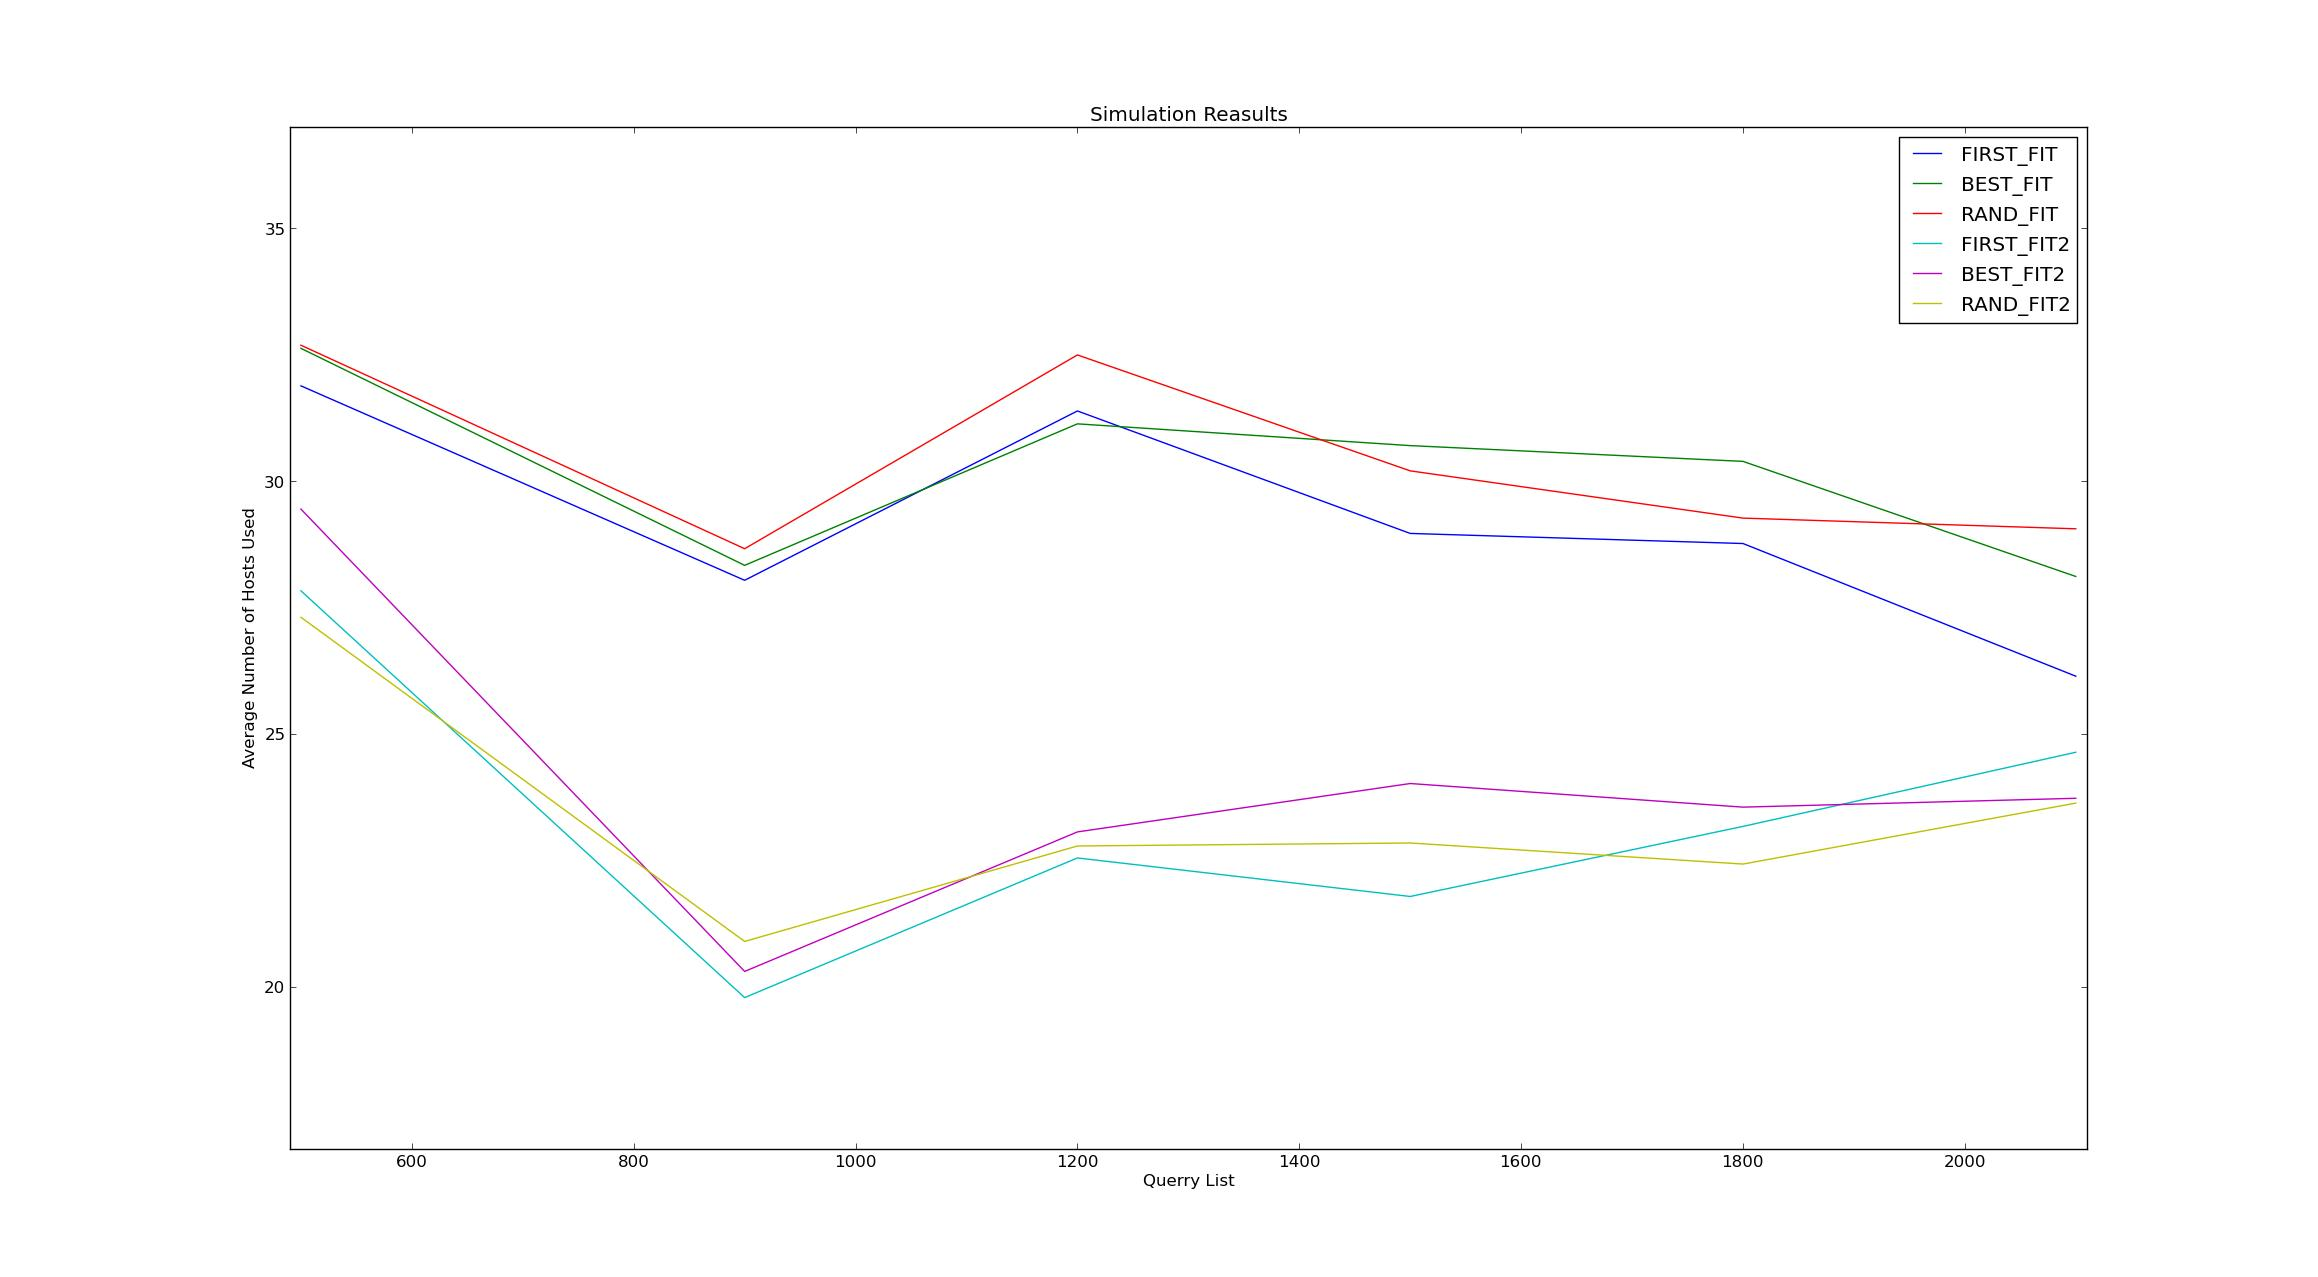
\includegraphics[width=1\textwidth]{7}
 \caption{Simulation Results}
 \end{figure}
}


\item{
\begin{figure}
  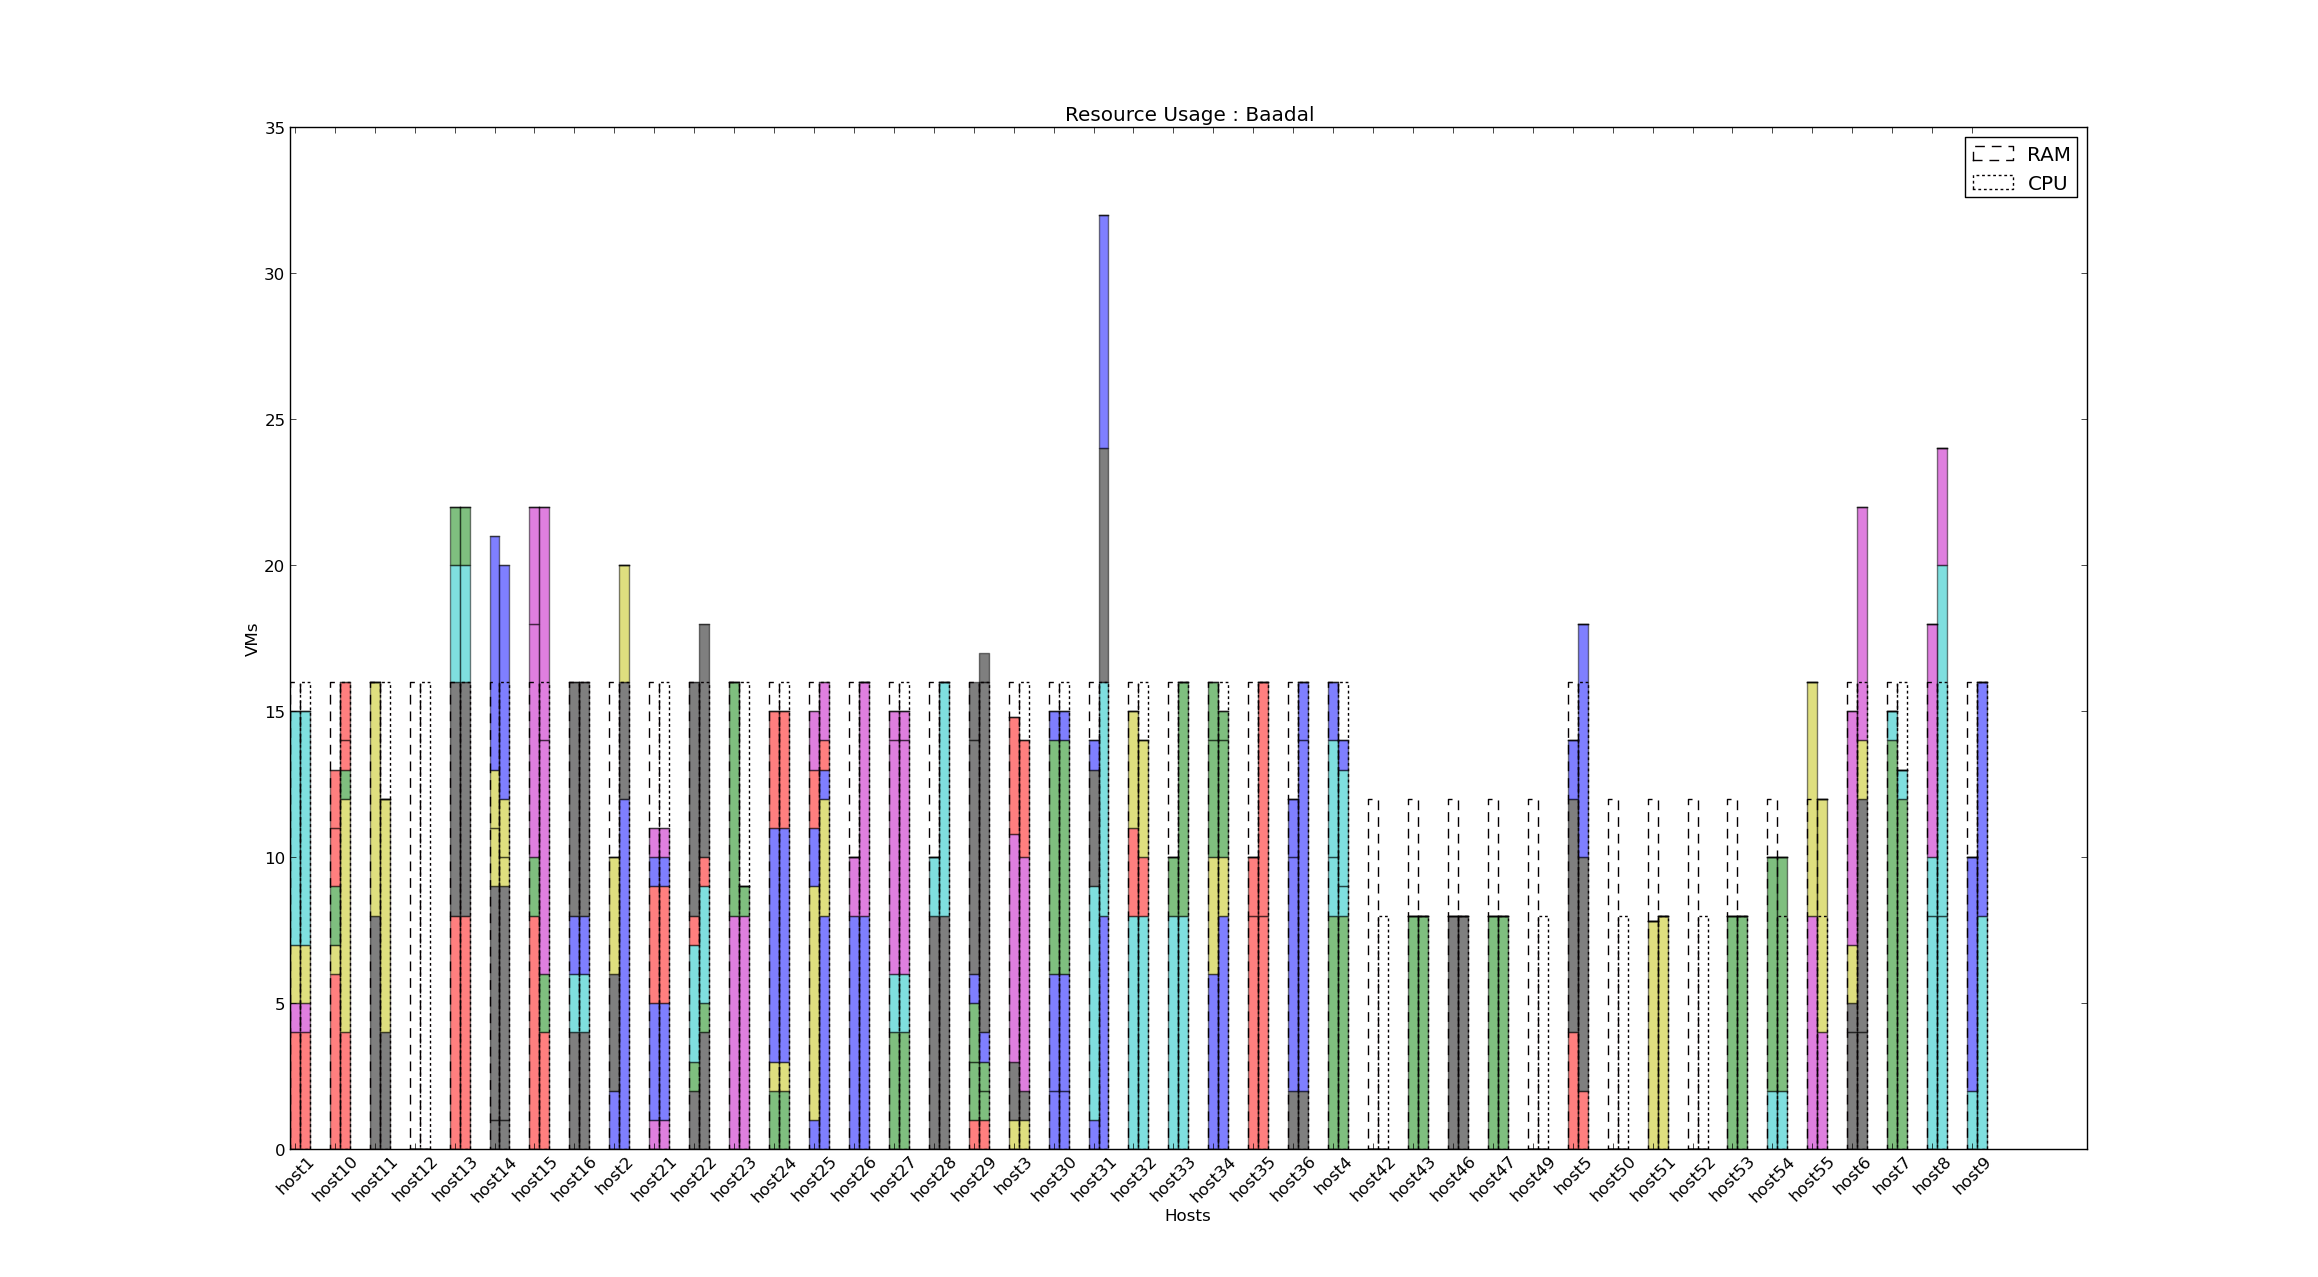
\includegraphics[width=1.1\textwidth]{h1}
 \caption{Initial State of Vms and Hosts}
 \end{figure}
 
 \begin{figure}
 \centering
  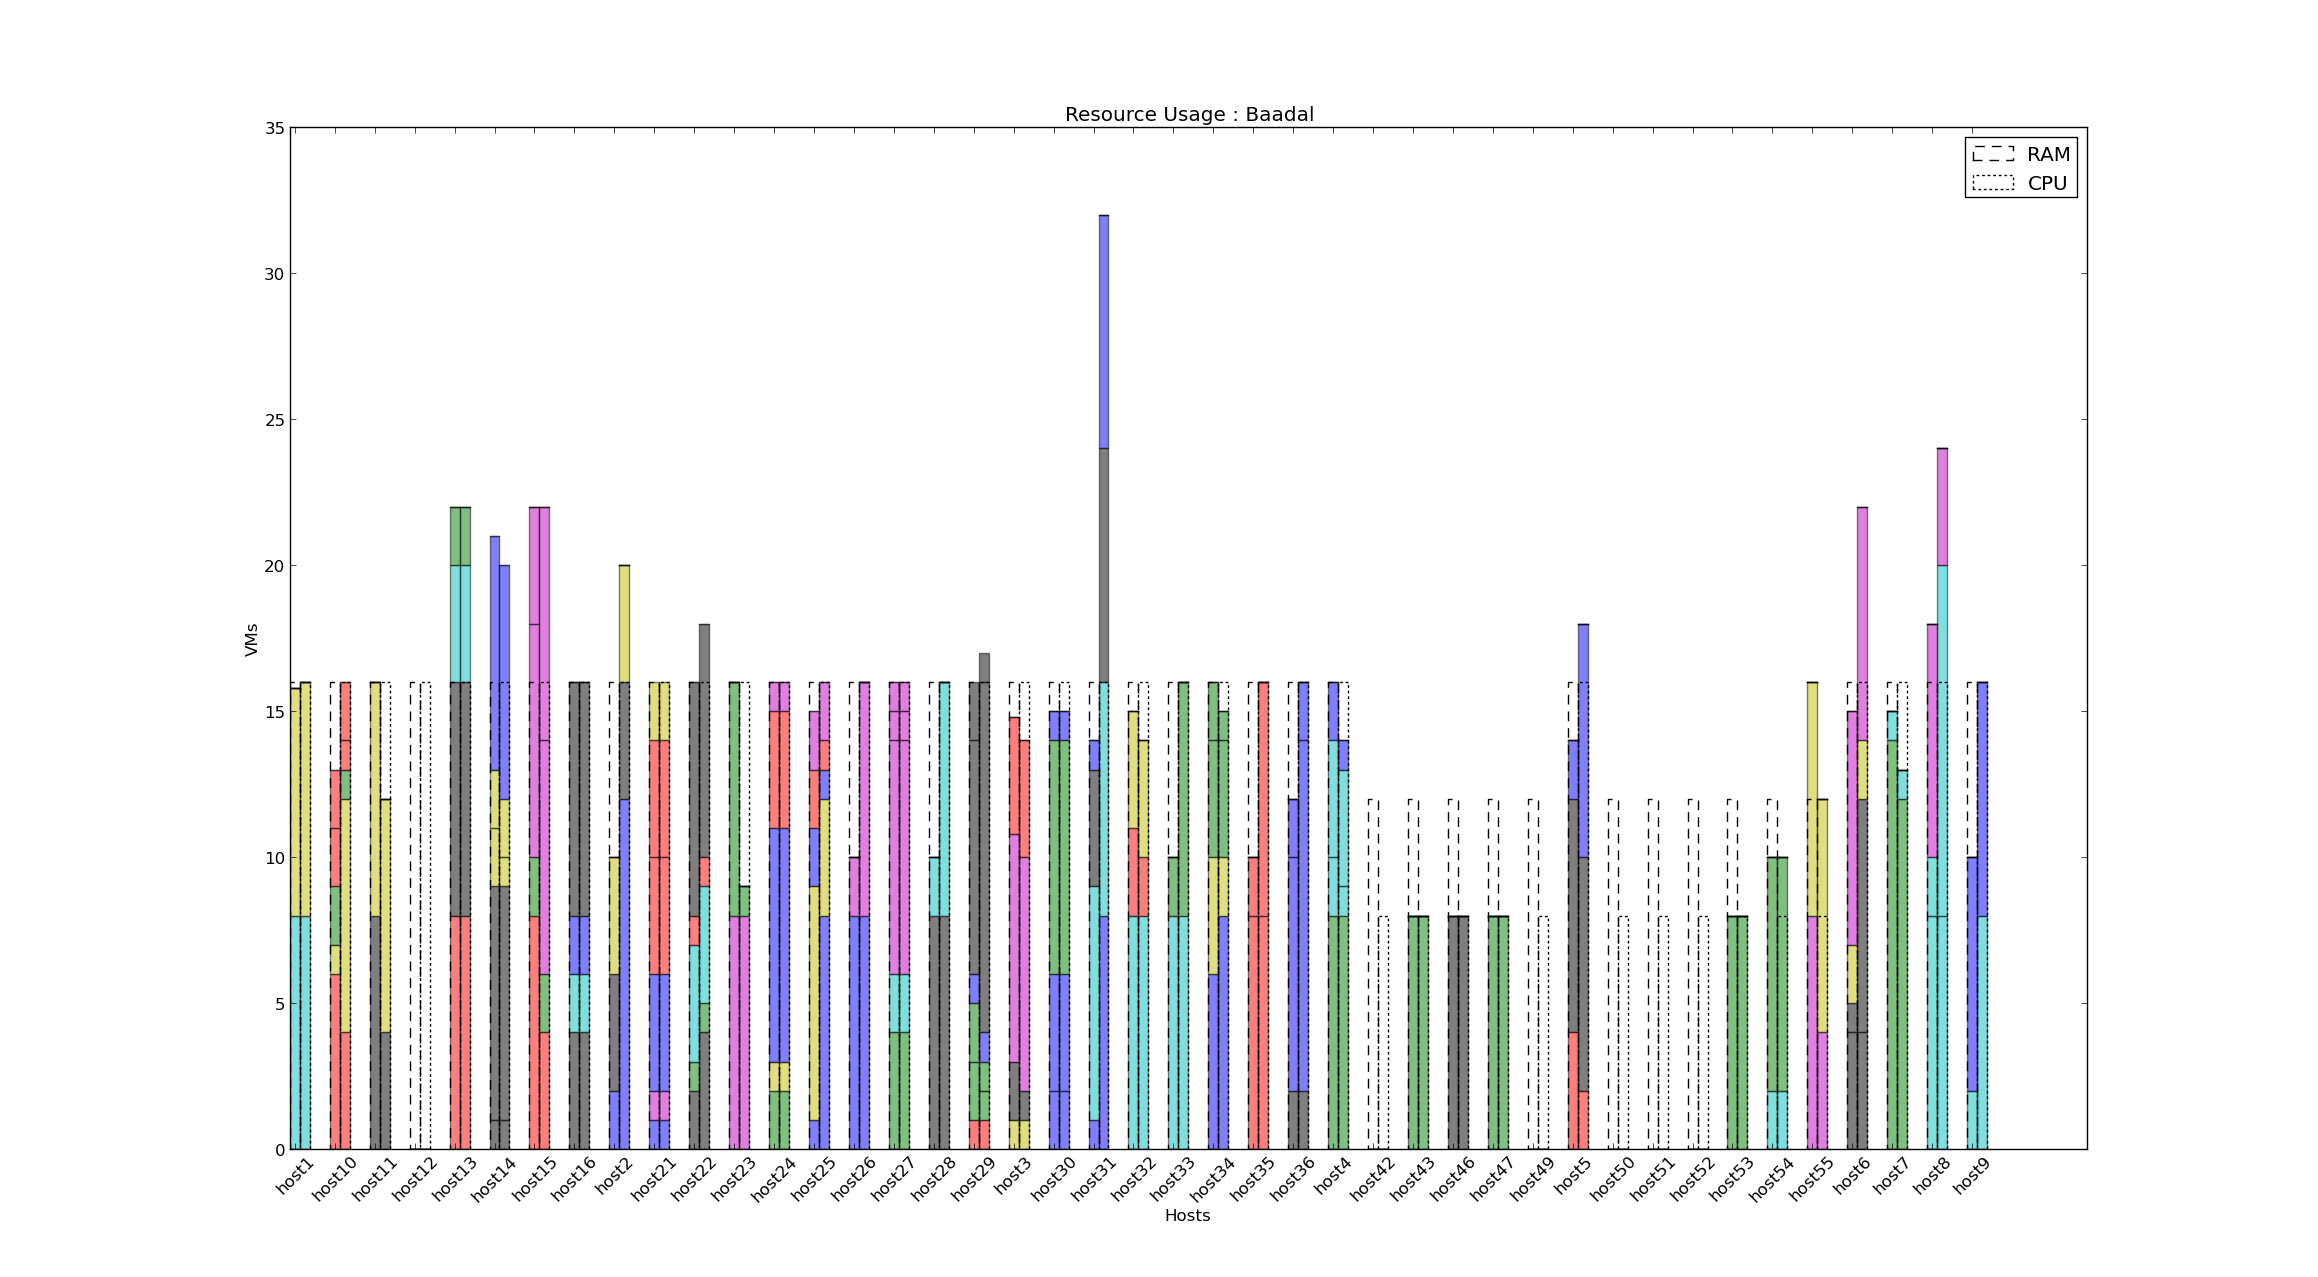
\includegraphics[width=1.1\textwidth]{h2}
 \caption{Host 51 shut down and its Vms migrated to other hosts}
 \end{figure}
}

\item{ We have also used migration if first fit fails to schedule a request to decrease the rejected requests during the simulation. The number of requests rejected for a list of 10,000 request were only 370 as compared to 665 without migration.
  }

\end{itemize}

\nocite{•}nocite{*}

\bibliographystyle{plain}
\bibliography{Baadal_rep}
\end{document}